\section{Lexical}

\begin{figure}[h]
    \centering
    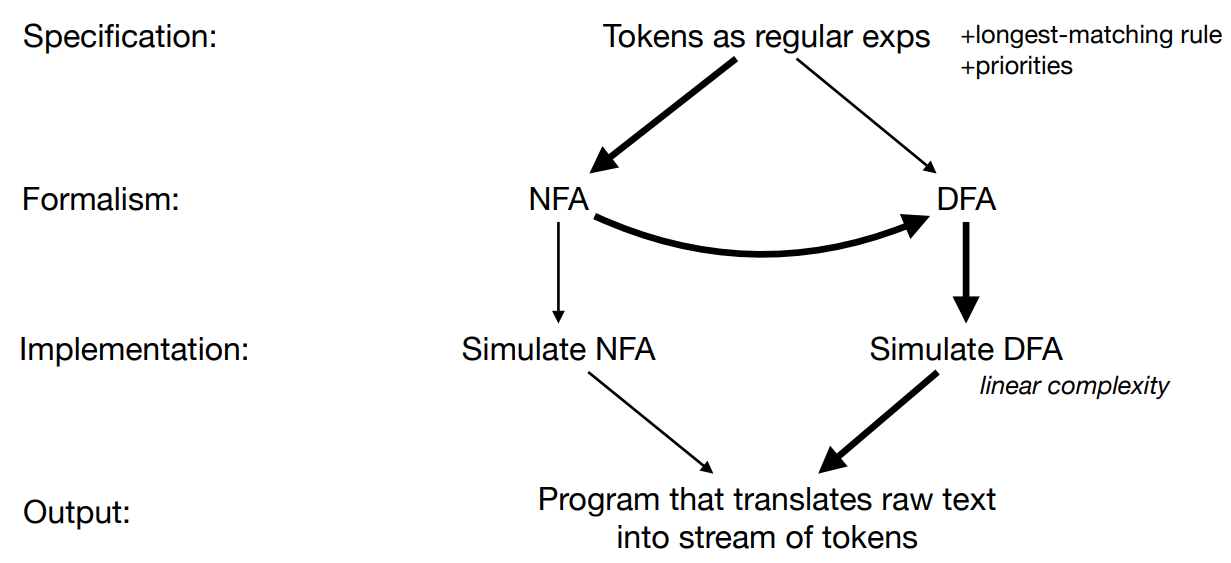
\includegraphics[scale=0.4]{assets/reg_nfa_dfa.png}
    \caption{REG to NFA to DFA}
    \label{fig:reg}
\end{figure}

\begin{itemize}
    \item Tokens: E.g. \textsc{ID}("a"), INT, IF etc. Some tokens include metadata like names in ID.
    \item Non-tokens: comments, whitespace etc.
    \item REG $\rightarrow$ NFA $\rightarrow$ (closures) DFA $\rightarrow$ Minimized DFA (more effective)
    \item REG: Handle priorities and longest matching string token wins.
    \item Ocamllex: Lexer generator
\end{itemize}